\section{安装HBase}
\subsection{简介}
HBase的设计来源于Google公司的BigTable论文,相当于是一个数据库,其查询的实时性较高。
也是Hadoop生态系统中的一个很重要的工具。

\subsection{配置文件}
\begin{lstlisting}[style=mysh, title=hbase-env.sh]
export JAVA_HOME=/opt/java
export HBASE_MANAGES_ZK=false
export HADOOP_HOME=/opt/hadoop
HBASE_CLASSPATH=$HBASE_CLASSPATH:$HADOOP_HOME/etc/hadoop
\end{lstlisting}
\lstinputlisting[style=myxml, title=hbase-site.xml]{docs/hbase/conf/hbase-site.xml}

我在配置HBase时,经常出现HMaster进程自动退出的问题,查看日志,调试了很长的时间。
多半是因为访问时权限的问题。可以在\lstinline{hdfs-site.xml}文件夹中加入
相应的权限设置选项,取消权限设置。

并且按照官网推荐,在HBase的配置目录下面,添加一个指向\lstinline{hdfs-site.xml}的
软连接。

启动HBase,需要先启动HBase服务。
\begin{lstlisting}[style=mysh, title=启动HBase]
$ start-hbase.sh
$ jps
# 使用Jps查看进程可以看到主节点上多了HMaster进程和HRegionServer进程
# 在从节点上多了HReginServer进程
# 如果出现过几秒后HMaster进程结束的情况,需要查看日志进行排查
\end{lstlisting}

\subsection{HBase Shell操作}
\begin{table}[htbp]
	\centering
	\caption{HBase操作指南}
	\begin{tabular}{p{4cm}|p{6cm}}
		\toprule
		操作 & 命令表达式 \\
		\midrule
		创建表 		& create "表名", "列族1", "列族2", \(\ldots\), "列族n"\\ \hline
		列出表 		& list \\ \hline
		获取表的描述 	& desc "表名" \\ \hline
		修改表 		& alter "表名" ,应先disable "表名"\\ \hline
		删除表 		& drop "表名" ,应先disable "表名"\\ \hline
		判断表是否存在 			& exists "表名"\\ \hline
		判断表是否是enable 		& is\_enabled "表名"\\ \hline
		判断表是否是disable 	& is\_disabled "表名"\\ \hline
		插入数据	& put "表名", "行键", "列族名:列名", "值" \\ \hline
		获取数据	& put "表名", "行键", "列族名:列名" \\ \hline
		全表扫描	& scan "表名" \\ \hline
		删除数据	& put "表名", "行键", "列族名:列名" \\ \hline
		查询行数	& count "表名" \\ \hline
		清空该表	& truncate "表名" \\ \hline
		更新表中数据	& 执行插入语句覆盖原来数据 \\ 
		\bottomrule
	\end{tabular}
	\label{tab:hbase_op}
\end{table}

下面是一些操作运行效果的截图:

\begin{center}
	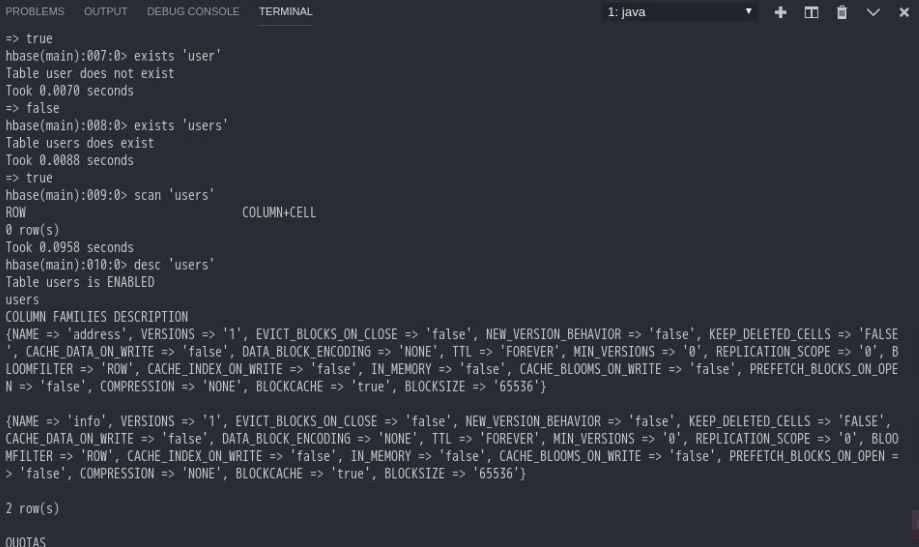
\includegraphics[width=\linewidth]{hbase/hbaseop2.png}

	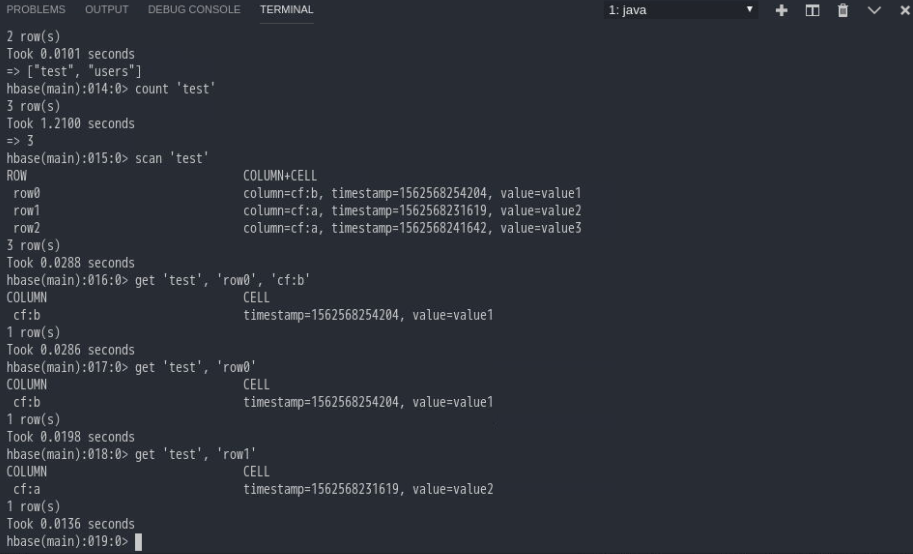
\includegraphics[width=\linewidth]{hbase/hbaseop1.png}

\end{center}

可以看出HBase的操作比较简单,这是其灵活性和扩展性的一种保障。

\subsection{HBase Java API使用}

HBase的Java API主要包括5大类的操作:HBase的配置、HBase表的管理、
列族的管理、列的管理、数据的操作。

\begin{enumerate}[1)]
	\item \lstinline{org.apache.hadoop.hbase.HBaseConfiguration}。
	
	HBaseConfiguration 类用于管理 HBase 的配置信息,使用举例如下。

\begin{lstlisting}[style=customjava]
static Configuration cfg = HBaseConfiguration.create();
\end{lstlisting}

\item \lstinline{org.apache.hadoop.hbase.client.Admin}

Admin 是 Java 接口类型,不能直接用该接口来实例化一个对象,而是必须通过调用 \lstinline{Connection.getAdmin()}方法,来调用返回子对象的成员方法。该接口用来管理 HBase 数据库的表信息。它提供的方法包括创建表,删除表,列出表项,使表有效或无效,以及添加或删除表列族成员等。

创建表使用的例子如下。

\begin{lstlisting}[style=customjava]
Configuration configuration = HBaseConfiguration.create();
Connection connection = ConnectionFactory.createConnection(configuration);
Admin admin = connection.getAdmin();
if(admin.tableExists(tableName)) {//如果存在要创建的表,那么先删除,再创建
	admin.disableTable(tableName);
	admin.deleteTable(tableName);
}
admin.createTable(tableDescriptor);
admin.disableTable(tableName);
HColumnDescriptor hd = new HColumnDescriptor(columnFamily);
admin.addColumn(tableName,hd);
\end{lstlisting}

\item \lstinline{org.apache.hadoop.hbase.HTableDescriptor}

\lstinline{HTableDescriptor}包含了表的详细信息。创建表时添加列族使用的例子如下。

\begin{lstlisting}[style=customjava]
HTableDescriptor tableDescriptor = new HTableDescriptor (tableName);// 表的数据模式
tableDescriptor. addFamily (new HColumnDescriptor("name"));// 增加列族
tableDescriptor.addFamily(new HColumnDescriptor("age"));
tableDescriptor.addFamily(new HColumnDescriptor("gender"));
admin.createTable(tableDescriptor);
\end{lstlisting}

\item \lstinline{org.apache.hadoop.hbase.client.Table}

Table是Java接口类型,不可以用 Table 直接实例化一个对象,而是必须通过调用\lstinline{connection.getTable()}的一个子对象,来调用返回子对象的成员方法。这个接口可以用来和 HBase 表直接通信,可以从表中获取数据、添加数据、删除数据和扫描数据。例子如下。

\begin{lstlisting}[style=customjava]
Configuration configuration = HBaseConfiguration.create();
Connection connection = ConnectionFactory.createConnection(configuration);
Table table = connection.getTable();
ResultScanner scanner = table.getScanner(family);
\end{lstlisting}


\item \lstinline{org.apache.hadoop.hbase.client.Put}

Put类用来对单元执行添加数据操作。给表里添加数据的例子如下

\begin{lstlisting}[style=customjava]
Configuration configuration = HBaseConfiguration.create();
Connection connection = ConnectionFactory.createConnection(configuration);
Table table = connection.getTable();
Put put = new Put ("*1111".getBytes());//—个 Put 代表一行数据,行键为构造方法中传入的值
put.addColumn("name".getBytes(),null,"Ghander".getBytes());//本行数据的第一列
put.addColumn("age".getBytes(),null,"20".getBytes());// 本行数据的第二列
put.addColumn("gender".getBytes(),null,"male".getBytes());// 本行數据的第三列
put.add("score".getBytes(),"Math".getBytes(),"99".getBytes());// 本行数据的第四列
table.put(put);
\end{lstlisting}


\item \lstinline{org.apache.hadoop.hbase.client.Get}

Get类用来获取单行的数据。获取指定单元的数据的例子如下。

\begin{lstlisting}[style=customjava]
Configuration configuration = HBaseConfiguration.create();
Connection connection = ConnectionFactory.createConnection(configuration);
Table table = connection.getTable();
Get g = new Get(rowKey.getBytes());
Result rs = table.get(g);
\end{lstlisting}


\item \lstinline{org.apache.hadoop.hbase.client.Result}

Result 类用来存放 Get 或 Scan 操作后的查询结果,并以\lstinline{<key,value>}的格式存储在映射表中。
获取指定单元的数据的例子如下。

\begin{lstlisting}[style=customjava]
Configuration configuration = HBaseConfiguration.create();
Connection connection = ConnectionFactory.createConnection(configuration);
Table table = connection.getTable();
Get g = new Get(rowKey.getBytes());
Result.rs = table.get(g);
for (KeyValue kv : rs.raw()) {
	System.out.printIn("rowkey:"+new String(kv.getRow()));
	System.out.printIn("Column Family:"+new String(kv.getFamily()));
	System.out.printIn("Column :"+ new String(kv.getQualifier()));
	System.out.printIn("value :"+ new String(kv.getValue()));
}
\end{lstlisting}


\item \lstinline{org.apache.hadoop.hbase.client.Scan}

Scan 类可以用来限定需要查找的数据,如版本号、起始行号、终止行号、列族、列限定符、返回值的数量的上限等。设置 Scan 的列族、时间戳的范围和每次最多返回的单元数目的例子如下。

\begin{lstlisting}[style=customjava]
Scan scan = new Scan();
scan.addFamily(Bytes.toBytes("columnFamily1"));
scan.setTimeRange(1,3);
scan.setBatch(1000);
\end{lstlisting}


\item \lstinline{org.apache.hadoop.hbase.client.ResultScanner}

ResultScanner类是客户端获取值的接口,可以用来限定需要查找的数据,如版本号、起始行号、终止行号、列族、列限定符、返回值的数量的上限等。获取指定单元的数据的例子如下。

\begin{lstlisting}[style=customjava]
Scan scan = new Scan();
scan.addColumn(Bytes.toBytes("columnFamily1"),Bytes.toBytes("column1")); 
scan.setTimeRange(1,3);
scan.setBatch(10);
Configuration configuration = HBaseConfiguration.create();
Connection connection = ConnectionFactory.createConnection(configuration);
Table table = connection.getTable();
try {
	ResultScanner resuitScanner = table.getScanner(scan);
	Result rs = resultScanner.next();
	for (; rs != null;rs = resultScanner.next()){
		for (KeyValue kv : rs.list()){
			System.out.printIn("--------------");
			System.out.printIn("rowkey:"+ new String(kv.getRow()));
			System.out.printIn("Column Family: "+ new String(kv.getFamily()));
			System.out.printIn("Column :" + new String(kv.getQualifier ()));
			System.out.printIn("value :"+ new String(kv.getValue()));
		}
	}
} catch (IOException e) {
	e.printStackTrace();
}
\end{lstlisting}
\end{enumerate}

下面演示一个具体的编程实例来学习如何使用HBase Java API解决实际问题。
在本实例中,首先创建一个学生成绩表scores,用来存储学生各门课程的考试成绩,然后向 scores 添加数据。

表 scores 的概念视图如图\ref{fig:scores1}所示,用学生的名字 name 作为行键,
年级 grade 是一个只有一个列的列族,score 是一个列族,每一门课程都是 score 的一个列,
如 english、math、Chinese 等。score 的列可以随时添加。

\begin{figure}[h]
	\centering
	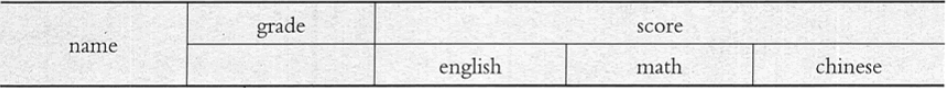
\includegraphics[width=\linewidth]{hbase/scores1.png}
	\caption{学生成缋表scores的概念视图}
	\label{fig:scores1}
\end{figure}

例如,后续学生又参加了其他课程的考试,如 computing、physics 等,
那么就可以添加到 score 列族。因为每个学生参加考试的课程也会不同,所以,
并不一定表中的每一个单元都会有值。在该实例中,要向学生成绩表 scores 中添加的数据如图\ref{fig:scores1}所示。

\begin{figure}[h]
	\centering
	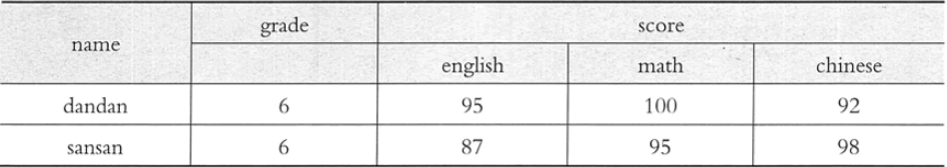
\includegraphics[width=\linewidth]{hbase/scores2.png}
	\caption{学生成缋表scores的数据}
	\label{fig:scores2}
\end{figure}

下面利用Maven和IDEA创建工程,在其中添加下面的依赖:

\begin{lstlisting}[style=myxml,title=添加Hbase Maven依赖]
<!-- https://mvnrepository.com/artifact/org.apache.hbase/hbase -->
<dependency>
	<groupId>org.apache.hbase</groupId>
	<artifactId>hbase</artifactId>
	<version>2.2.0</version>
	<type>pom</type>
</dependency>	
\end{lstlisting}

新建主程序,写入下面代码框架:

\begin{lstlisting}[style=customjava,title=主程序框架]
import java.io.IOException;
import org.apache.hadoop.conf.Configuration;
import org.apache.hadoop.hbase.*;
import org.apache.hadoop.hbase.client.*;
import org.apache.hadoop.hbase.util.Bytes;
public class StudentScores {
	public static Configuration configuration; //HBase 配置信息
	public static Connection connection; //HBase 连接
	public static void main (String [] agrs) thorws IOException{
		init();//建立连接
		createTable();//建表
		insertData();//添加课程成绩
		insertData();//添加课程成绩
		insertData();//添加课程成绩
		getData();//浏览课程成绩
		close();//关闭连接
	}
	public static void init () {......} //建立连接
	public static void close () {......} //关闭连接
	public static void createTable (){......} //创建表
	public static void insertData () {......} //添加课程成绩
	public static getData() {......} //浏览操程成绩
}
\end{lstlisting}

然后分别实现下面的几个函数:

\begin{lstlisting}[style=customjava,title=init函数,用于初始化连接]
public static void init() {
	configuration = HBaseConfiguration.create();
	configuration.set("hbase.rootdir", "hdfs://ldcluster:8020/hbase");
	try {
		connection = ConnectionFactory.createConnection(configuration);
		admin = connection.getAdmin();
	} catch (IOException e) {
		e.printStackTrace();
	}
}
\end{lstlisting}

\begin{lstlisting}[style=customjava,title=close函数,用于结束断开连接]
public static void close() {
	try {
		if (admin != null) {
			admin.close();
		}
		if (connection != null) {
			connection.close();
		}
	} catch (IOException e) {
		e.printStackTrace();
	}
}
\end{lstlisting}

\begin{lstlisting}[style=customjava,title=createTable函数]
public static void createTable(String myTableName, String[] colFamily) throws IOException {
	TableName tableName = TableName.valueOf(myTableName);
	if (admin.tableExists(tableName)) {
		System.out.println("The " + myTableName + "exists!");
	} else {
		HTableDescriptor hTableDescriptor = new HTableDescriptor(tableName);
		for (String str :
				colFamily) {
			HColumnDescriptor columnDescriptor = new HColumnDescriptor(str);
			hTableDescriptor.addFamily(columnDescriptor);
		}
		admin.createTable(hTableDescriptor);
	}
}
\end{lstlisting}

\begin{lstlisting}[style=customjava,title=向表中插入数据的函数]
public static void insertData(String tableName, String rowKey, String colFamily, String col, String val) throws IOException {
	Table table = connection.getTable(TableName.valueOf(tableName));
	Put put = new Put(rowKey.getBytes());
	put.addColumn(colFamily.getBytes(), col.getBytes(), val.getBytes());
	table.put(put);
	table.close();
}
\end{lstlisting}

\begin{lstlisting}[style=customjava,title=从表中获取数据的函数]
public static void getData(String tableName, String rowKey, String colFamily, String col) throws IOException {
	Table table = connection.getTable(TableName.valueOf(tableName));
	Get get = new Get(rowKey.getBytes());
	get.addColumn(colFamily.getBytes(), col.getBytes());
	Result result = table.get(get);
	System.out.println(new String(result.getValue(colFamily.getBytes(), col.getBytes())));
	table.close();
}
\end{lstlisting}

完整的主函数如下:

\begin{lstlisting}[style=customjava,title=完整的主函数]
public static void main(String[] args) throws IOException {
	String tableName = "scores";
	String[] colFamily = {"grade","score"};

	init();
	createTable(tableName, colFamily);
	insertData(tableName, "dandan", "grade", "","6");
	insertData(tableName, "dandan", "score", "english", "95");
	insertData(tableName, "dandan", "score", "math", "100");
	insertData(tableName, "dandan", "score", "chinese", "92");

	insertData(tableName, "sansan", "grade", "","6");
	insertData(tableName, "sansan", "score", "english", "87");
	insertData(tableName, "sansan", "score", "math", "95");
	insertData(tableName, "sansan", "score", "chinese", "98");

	getData(tableName, "dandan", "score", "math");
	getData(tableName, "sansan", "score", "english");
	getData(tableName, "sansan", "grade", "");

	close();
}
\end{lstlisting}

运行结果如下:

\begin{center}
	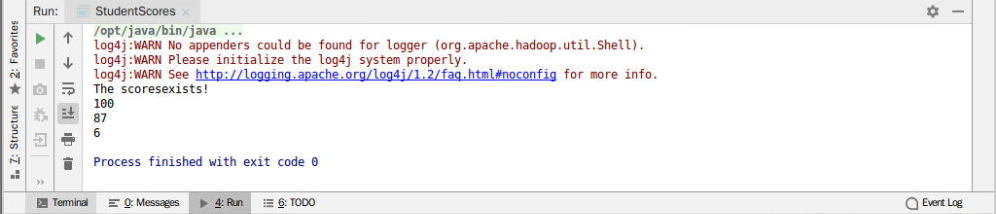
\includegraphics[width=\linewidth]{hbase/output.png}

	可以在控制台看到输出的结果,但是需要运行等待的时间较长。

	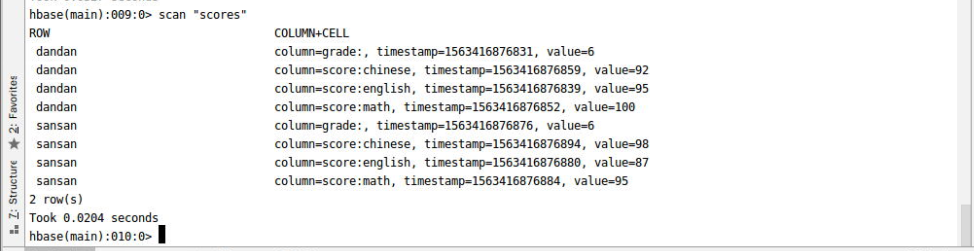
\includegraphics[width=\linewidth]{hbase/scan.png}

	在Hbase shell中也可以看到表的信息
\end{center}

总结:采用HBase Shell操作的实时性较好,但是灵活性不够,适合演示或小量数据。
而采用Java API编程能够加深对HBase各个模块的理解,而且更加灵活,适合各种复杂大数据量情况。

